sud%\title{X}Experiment Report
\documentclass[12pt,letterpaper]{article} %document type and other specifications
\usepackage[utf8]{inputenc} %To write tildes and ñ
%\usepackage[spanish]{babel} %For the titles of figures, tables and others are in Spanish
%\addto \captionsspanish{\renewcommand{\tablename}{Table}} %Rename tables
%\addto \captionsspanish{\renewcommand{\listtablename}{Index}} %tables Rename tables list
\usepackage{geometry}                         
\geometry{left=18mm,right=18mm,top=21mm,bottom=21mm} %Size writing area of the page
\usepackage{ucs}
\usepackage{amsmath}    %ams packages developed by the American Mathematical Societ
\usepackage{amsfonts}   %and improve writing formulas and mathematical symbols
\usepackage{amssymb}
\usepackage{graphicx}   %To insert graphics
\usepackage[lofdepth,lotdepth]{subfig}	%To place several figures
\usepackage{unitsdef}	%For proper presentation of unit
\usepackage{pdfpages}   %include pdf pages external to the Annexes
\usepackage{appendix}   %for attachments
\renewcommand{\unitvaluesep}{\hspace*{4pt}}	%Resizing the size and spacing unit
\usepackage[colorlinks=true,urlcolor=blue,linkcolor=black,citecolor=black]{hyperref}     %to insert hyperlinks and bookmark
\usepackage{float}		%To locate tables and figures just after the text
\usepackage{booktabs}	%To make stylized table
\batchmode
\bibliographystyle{plain} 
\pagestyle{plain} 
\pagenumbering{arabic}
\usepackage{lastpage}
\usepackage{fancyhdr}	%To handle headers and foote
\pagestyle{fancy}		%content of headers and footer
\usepackage{multicol}   %for multiple columns

%------------------------ Definition of abstract environment ------------------------%
\newcounter{resumen}
\setcounter{resumen}{0}
\def\theejemplo{\thechapter.\arabic{resumen}}

\newenvironment{resumen}
{	
	\begin{center}
	\begin{minipage}[t]{500 pt}
	\vspace{5mm}
	\emph{\textbf{RAbstract}}
	\\[-2mm]
	\line(1,0){500}
	\\[-4.25 mm]
	\line(1,0){500}
	\\
}
{
	\normalsize
	\\[2mm]
	\footnotesize\textbf{Keywords: \footnotesize\@palabras}
	\\[-2mm]
	\line(1,0){500}
	\\[0.5cm]
	\end{minipage}
	\end{center}
}

%-------------------- For keywords --------------------%
\def\palabras#1{\gdef\@palabras{#1}}

%%%%%%%%%%%%%%%%%%%%%%%%%%%%%%%%%%%%

\lhead{AE 230 - Modelling and Simulation Laboratory}
\chead{}
\rhead{Experiment 1}	% Here is the number of experiment, as in the title
\lfoot{Aerospace Engineering}
\cfoot{\thepage\ of \pageref{LastPage}}
\rfoot{IIT Bombay}


\author{{\small Group 11} \\ Kunal Tyagi, 120010006 \\ Kuldeep Singh, 120010 \\ Pratibha Ojwani, 120010 \\ A Nitin Kumar, 12001 \\ \vspace*{3.0in} }

\title{Indian Institute of Technology, Bombay\\{\small Aerospace Engineering\\Ae 230 Modelling and Simulation Laboratory\\ \vspace*{0.55in} Report}\\ Experiment 1\vspace*{1.35in}}
\date{}  				

%%%%%%%%%%%%%%%%% Keywords
\palabras{Wind Tunnel, blah blah}
%%%%%%%%%%%%%%%%%
%Are written after the abstract and synthesize the fundamental concepts of the experiment as a label


%%%%%%%%%%%%%%%%
\begin{document}	%Top of Document
%%%%%%%%%%%%%%%%

\pdfbookmark[1]{Home}{home} 	%Bookmark for Title

\maketitle							% Title


\tableofcontents
\newpage
\listoffigures
\listoftables

\newpage
\section{Abstract}
%%%%%%%%%%%%%%%%%%%
\begin{resumen}
This section describes the experiment and how they develop concis way, with emphasis on results and important conclusions in a maximum of 160 words is described.
\end{resumen}
%%%%%%%%%%%%%%%%%%%


%%%%%%%%%%%%%%%%%%%
\section{Objectives}
%%%%%%%%%%%%%%%%%%%

\subsection{Aim}
%%%%%%%%%%%%%%%%%%%%%%%%%%%%%

Objective described in Experiment Guide.


\subsection{Specific objectives}
%%%%%%%%%%%%%%%%%%%%%%%%%%%%%%%%%%

\begin{itemize}
\item Specific objectives proposed by students .
\item They are comprehensive and based on theoretical note, the procedure and the expected results of the experiment.
\end{itemize}

\newpage

%%%%%%%%%%%%%%%%%%%%%%%%%%
\section{List of equipment}
%%%%%%%%%%%%%%%%%%%%%%%%%%

The list of equipment used in the experiment shown in Table \ref{T:equipment}.

\begin{table*}[!ht]
\caption{List of equipment}
\label{T:equipment}
\begin{center}
\begin{tabular}{| c | c | c | c | c | c | c |}
\hline
\textbf{Equipment} & \multicolumn{3}{| c |}{\textbf{Sesión 1}} & \multicolumn{3}{| c |}{\textbf{Sesión 2}} \\ 
\cline{2-7}
& \textbf{Brand} & \textbf{Model} & \textbf{Plate} & \textbf{Brand} & \textbf{Model} & \textbf{Plate} \\
\hline
Source DC &&&&&& \\
Digital oscilloscope &&&&&& \\
Signal generator &&&&&& \\
Multifunction Meter &&&&&& \\
Breadboard &&&&&& \\
\hline
\end{tabular}
\end{center}
\end{table*}

\newpage

%%%%%%%%%%%%%%%%%%%%%%%%%%%%%
\section{List of components}
%%%%%%%%%%%%%%%%%%%%%%%%%%%%%

The list of components used in the experiment shown in Table \ref{T:components}.

\begin{table*} [!ht]
\caption{Lista de componentes}
\label{T:components}
\begin{center}
\begin{tabular}{| c | c | c | c | c | c |}
\hline
\textbf {Component} & \textbf {Symbol} & \textbf {Face value} & \textbf {Measured value} & \textbf {Tolerance} & \textbf {Power } \\
\hline
Resistor cerámico & R1 & \kiloohm[1] & &  & 0,25 W\\ 
Potenciómetro & Rp & \kiloohm[5] & &  & 2 W\\
Capacitor electrolítico & C11 & 150\microfarad & & - & - \\ 
Capacitor cerámico & C & 100\nanofarad & & - & - \\
Diodo & 1N4148 & & & & 500 mW\\
Transistor BJT & 2N2222A & & & & 1000 mW\\
\hline
\end{tabular}
\end{center}
\end{table*}


\newpage
%%%%%%%%%%%%%%%%%%%%%%%
\section{Experimental Results and analysis of results}
%%%%%%%%%%%%%%%%%%%%%%%
Yeah, but how 

\newpage
%%%%%%%%%%%%%%%%%%%%%%%
\section{Conclusions}
%%%%%%%%%%%%%%%%%%%%%%%


%%%%%%%%%%%%%%
% Bibliography
%%%%%%%%%%%%%%

\newpage

The recommended format is the APA bibliography . The following is an example :

\begin{thebibliography}{}
\bibitem[Apuntes, 2008]{apuntes} \emph{http://www.apuntesdeelectronica.com/componentes/transistor-igbt.htm} consultado el 12/05/2013.
\bibitem[Boylestad, 1998]{Boylestad} Robert L. Boylestad, Louis Nashelsky (1998). \emph{Electronic Devices and Circuit Theory}. New Jersey:  Pearson Prentice Hall, 7th Edition.



\end{thebibliography}


\newpage

%%%%%%%%%%%%%%
% Annexure
%%%%%%%%%%%%%%

\appendix
\section{Appendices}

Includes information sheets manufacturer of components used or any other information deemed necessary .

The following is a way to attach pages as PDFs sheets manufacturer, but there are many ways to attach the annexes as deemed necessary .

%%%%% Transistor NTE123A y NTE159M
\subsection{Transistor 2N2222A}
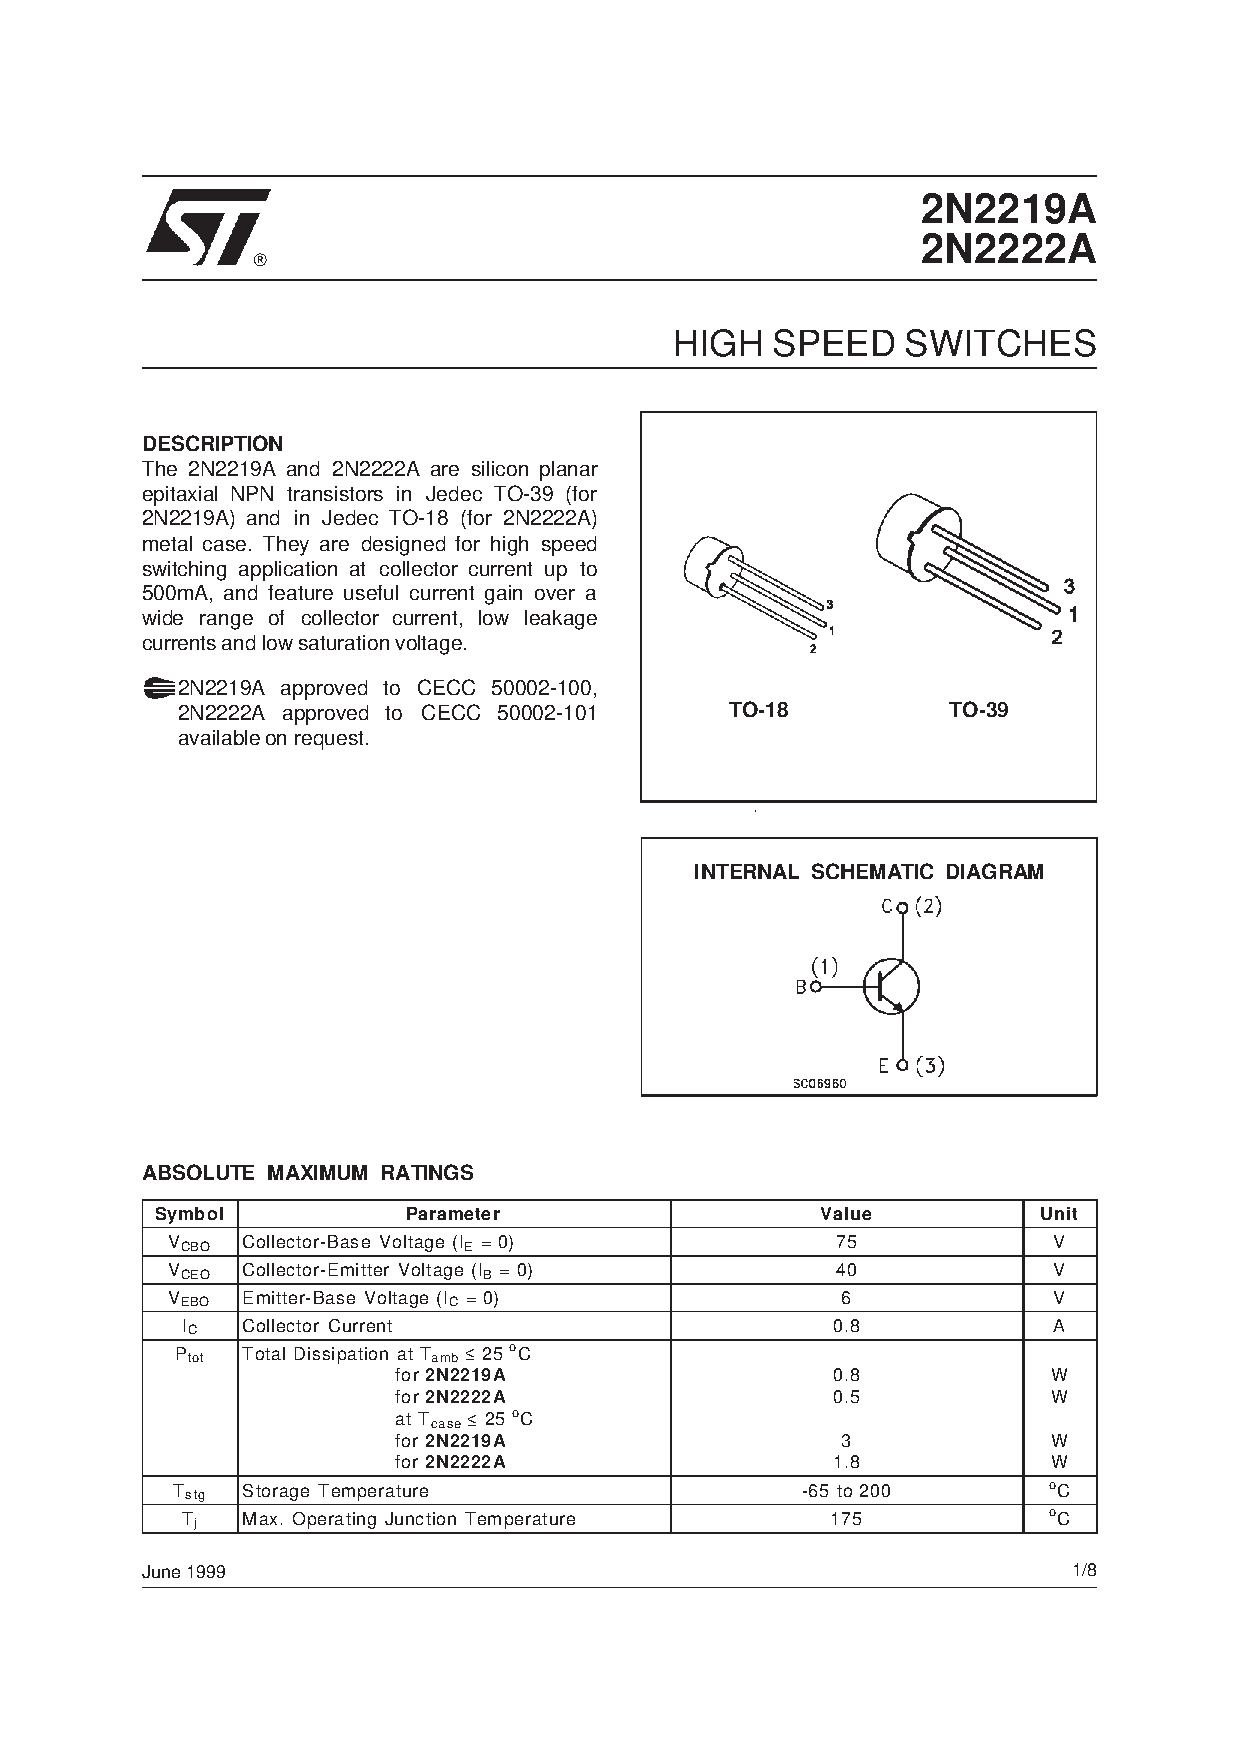
\includepdf[pages={1-3}]{./annexes/2N2222A.pdf}



%%%%%%%%%%%%%%
\end{document}
%%%%%%%%%%%%%%